% compiling and viewing latex in os x
% brew cask install mactex
% /Library/TeX/texbin/pdflatex main.tex 

\documentclass{article}
\usepackage[T1]{fontenc}
\usepackage[utf8]{inputenc}
% \usepackage{lmodern}

\usepackage{listings}
\usepackage{float}
\title{GPUcoin decentralized uncensorable open source distributed computing, live-streaming Protocol and Marketplace Technical Whitepaper}
\author{GPUcoin Protocol Team}
% \date{July 26 2017}
\date{\today}
\setlength{\parskip}{1em}
\usepackage{natbib}
\usepackage{graphicx}
\usepackage{amssymb}
\usepackage{amsmath}
\usepackage{nameref}
\usepackage[normalem]{ulem}
% \usepackage{soul}
\usepackage[table]{xcolor}
\usepackage{tabularx}
\usepackage{adjustbox}
\usepackage[english, status=draft]{fixme}
\fxusetheme{color}
\renewcommand\tabularxcolumn[1]{m{#1}}% for vertical centering text in X column

\begin{document}

\maketitle

\begin{abstract}
The GPUcoin team is building the next generation technology for live streaming and distributed computing services based on blockchain technology and a new innovative open source decentralized GPU live-streaming and distributed computing protocol that would eliminate expensive content delivery networks and use peer-to-peer nodes for delivering not just live-streaming video but also archived videos. This platform can be generalized to build a web scale cryptographically secure distributed computing environment creating the world;s first \textbf{I}nterplanetary \textbf{C}ompute \textbf{N}etwork(IPCN). A peer-to-peer hyperstream protocol that makes live-streaming and distributed computing on GPUs secure, faster, safer, and open.

\iffalse
\sout{We will use crypto-financing (Initial Coin Offering) for capital rather than traditional venture capital and shareholders.}
\fi

\end{abstract}
\newpage

\tableofcontents
\newpage

\section{Introduction}
\subsection{History of Live-Streaming}
Over the last half a century, people have been fascinated by live video. On September 4, 1951, Harry Truman spoke at the Japanese Peace Treaty Conference in San Francisco and, this was the worlds first live broadcast. Four months later, The Today Show would become the first broadcast news program airing live in the United States. Since then, we have loved live video, from our favorite news stations to our guilty pleasures of reality television.

\iffalse
\sout{Streaming is a lot older in its origins than one might intuitively suppose. One of the earliest streaming platforms was Muzak. This along with similar audio systems played continuous music. When we think of streaming, though, we think computers and the Internet. The full development of that capacity was more recent. Many technical advances in the 1990s and 2000s improved the bandwidth of networks. This increased the number of people and computers with access to those networks, creating the Internet as we know it today. Standard formats were also developed and protocols that we use to code online material and functions (TCP/IP, HTTP, HTML, etc.).}
\fi

As the bandwidth of connections to the Internet and computing power available to the average person continued to increase, it was natural that the audio streaming used by Internet radio would graduate to streaming video. Data compression methods contributed a lot to this development as well. Video files contain a lot of information. Compression allows that information to be efficiently transmitted and stored.

\subsection{Live-Streaming versus On-Demand Streaming}
The term “live-streaming” is sometimes applied where it doesn’t belong. Streaming from a recorded source, which is what one finds on YouTube, Netflix, and many other commercial streaming sources, is on-demand streaming. This means that the user can watch the content at will, while live-streaming occurs only at the moment, in real-time. Live streaming comes from a content source such as video cameras and microphones. It is made available at the same time as the event being filmed occurs. On-demand streaming provides content from a recorded source instead. Streaming radio and much Internet television consists of live-streaming. As far as the “streaming” portion of the process is concerned, live and on-demand streaming are similar from the viewer’s perspective. They are quite different in technical and procedural details from the standpoint of the producer or broadcaster, though. The main difference from a technical end is the use of temporary storage for the material in progressive streaming or on-demand streaming. This is where a file is partially downloaded, stored to memory, and played while the next portion of the file is downloading. True streaming or live-streaming does not employ partial memory capture. It streams directly from the source to the user via a computer processor that finalizes the broadcast.

\section{Bitcoin, Ethereum, Blockstack, Toshi, Status \& the decentralized web revolution}
 The internet is in the middle of the august beginnings of decentralization revolution: centralized proprietary services are being replaced with \textbf{decentralized open ones with open source code}; trusted parties replaced with \textbf{verifiable mathematical computation}; brittle location addresses replaced with \textbf{resilient content addresses}; inefficient monolithic services replaced with \textbf{peer-to-peer algorithmic markets} ; complex inefficient unverifiable data-structures with \textbf{verifiable efficient data-structures, Merkle Trees}. Bitcoin, Ethereum, and other blockchain networks have proven the utility of decentralized transaction ledgers. These public ledgers process sophisticated smart contract applications and transact crypto-assets worth tens of billions of dollars every day. These systems are the first instances of internet wide open services, where participants form a decentralized network providing useful services for pay, with no central management or trusted parties.
Virtually none of the ideas underpinning Bitcoin are new. They can all be traced to the academic literature going back decades.

 Cryptographic signatures and public-key cryptography, cryptographic hash functions, cryptographic proof-of-work, time-stamping, Merkle trees, chains of transactions blocks, Byzantine fault tolerance, smart contracts - all of these ideas were old when Bitcoin was invented.
 Satoshi Nakamoto's achievement lays in the complex, ingenious way in which he (or she, or they) combined these ideas into a new distributed algorithm\footnote{http://queue.acm.org/detail.cfm?id=3136559}.
 
\textbf{Netscape moment}: \emph{Cambrian} explosion of crypto-currency Ðapps
 
% \newcolumntype{Y}{>{\centering\arraybackslash}X}

 \begin{adjustbox}{width=.75\textwidth}
\begin{tabularx} {\textwidth}{|X|X|X|X|}
 \hline
& 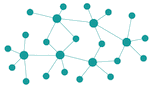
\includegraphics[scale=0.2]{static/decentnew} & 
\includegraphics[scale=0.2]{static/hootcoin} & \\
 \hline
\textbf{Phase} & \textbf{Internet} & \textbf{Crypto-currency} & \textbf{Reach}\\
\hline
Protocol & TCP/IP, SMTP & bitgold, \textbf{Bitcoin}, Ethereum & 1M People \\
\hline
Infrastructure & ISPs, lay fiber & \textbf{Exchanges}, secure storage & 10M people \\
\hline
Consumer Interface & Browser & User controlled \textbf{btc/eth wallets} & 100M people \\
\hline
Decentralized Ðapps & Web 2.0 & Finance 2.0 Ðapps & 1B people\\
\hline
Fat Protocols & Web 3.0 & Filecoin, \textbf{GPUCoin ICO} empower next-gen Ðapps & 2B people\\

\hline
\end{tabularx}
\end{adjustbox}

Protocol layer like \textbf{File}-coin and \textbf{GPU}-Coin ICO is the next Web 3.0

Firefox, Chrome and IE have dominated the centralized web. decentralized technologies such as Blockstack are ushering in the auspicious beginnings of decentralized web. 
We are now entering a new era of decentralized applications, blockchain technologies collectively known as Web 3.0. In the centralized web, the users are the product, their interests, preferences are sliced and diced by companies such as Facebook, Twitter and Google and sold to advertisers, enriching their small group of shareholders driven by profit, with significant barriers to entry. In the
decentralized web, the user information is private and value creation is not about advertisements and shareholder enrichment only. Decentralized
technologies such as Status, Toshi and Hoot empower the network token holders, who can have many motivations other than mere profit, including privacy, altruism and a more inclusive distribution of control and information. The emergence of bitcoin and subsequent blockchain technologies has generated a new digital asset class in which scarcity is based on mathematical properties and equations rebalancing variables to maximize economic inclusivity and activity. Through cryptographic verification and game-theory based equilibrium, blockchain-based digital assets can be created, issued, and transmitted using software. Ownership of these cryptographic digital assets can be easily verified using public key cryptography and transfer of ownership maintained in an immutable decentralized distributed database ledger known as the blockchain. This lays the foundation for democratic transfer of value among entities in the decentralized web.
We are in the very early big-bang stages of the crypto-currency decentralized web revolution on blockchain and several miracles are happening everyday harkening to the early merry days of web 1.0.

\section{Motivation - design goals}
In our development of Hoot, we aspire to address four problems with live streaming and compute over blockchain:
\begin{itemize}
\item[-]Entertainment systems are designed to benefit the select few in Hollywood, most artists, musicians and creators have little or no access to the monetary benefits of their own creations.
\item[-]internet service providers such as AT\&T, Comcast and verizon slow down or block any content, applications or websites you may use
\item[-]Most video and live systems are centralized subject to central censorship, leading to citizens unwilling or unable to share their free speech openly
\item[-]As the systems to deploy video and live are expensive and centralized there has been a significant lack of innovation.
\item[-]Monetization systems are also very rudimentary with annoying intrusive advertisements that are hard to avoid during video experiences. 
\end{itemize}


We believe a more egalitarian and democratic open Hoot GPUcoin marketplace is the panacea to many of the problems the old systems fail to address:
\begin{itemize}
\item[+]By giving creators a way to monetize their own creations on Hoot, we empower them to create, trusting the open decentralized marketplace to fairly compensate them over archaic centralized controlled channels.
\item[+]\textbf{Net Neutrality}: we strongly support and believe in net neutrality and by design the hoot GPUCoin decentralized net prevents any form of throttling, blocking or slowing down content.
\item[+]By making the video system decentralized and uncensorable, Hoot promotes citizen free speech without risk of detection and censorship
\item[+]By making video and compute systems more expressive we plan to make video systems democratic and uncensorable, leading to an unleashing of video innovation on the open decentralized web.

\item[+]By making the platform opensource and decentralized over the blockchain, creators can price their content and accept cryptocurrencies in place of intrusive advertisements which only benefit centralized systems such as facebook, making this a more seamless experience for end consumers. Since cryptocurrencies do not need to be issued by a central authority, financial means of control to censor content is made irrelevant. Blocking a payment channel is a common means of censorship e.g., the paypal banking account belonging to Wikileaks was blocked by various central controlling organizations.
\end{itemize}

% \fxerror{need to combine all problems or delete $2/3$}

\subsection{Customer Business Problem}
The consumer world is ready for mobile live broadcasting. Participation in a live-stream is the next big wave and future of interactive live TV. Facebook serves about 8 Billion video views a day and Snapchat about 10 Billion. Current mobile live-steaming apps do not deliver true real-time, failing in typical real world mobile use cases where high bandwidth and battery usage is unacceptable. Consumers also lose their memorable moments as the live-streams are ephemeral. eSports such as \emph{Dota2} are very popular among gamers and live-streaming audiences alike. The e-sporting events constantly draw audiences in the millions comparable to live football and baseball sporting events. Being able to stream to millions of viewers with near zero latency and HD quality has been a huge challenge for the existing CDN based live-streaming systems.

\subsection{Solution to customer problem / Product Offering}
A consumer grade true real-time live-streaming service needs to be
built from the ground up to offer live-streaming of mobile games and eSports, for iPhone, iPad, Android smartphones and tablets. Hoot's break through open source live-streaming technology brings true real-time video in a scalable way to its audience, with just the network latency. Hoot smart mobile streaming, being self adaptive based on network conditions and available bandwidth, results in significantly lower bandwidth and battery consumption, leading to superior user experience. Hoot also allows users to stream from their Mac/PC devices, in addition to the mobile apps, directly to engage their social audience. Hoot is the best way to watch, broadcast interactive live-stream videos and discover talented broadcasters.

% \section{Mission}
% Hoot Mission
% \fxerror*{need to enter Hoot mission or delete}
%
% \section{Vision}
% Hoot Vision
% \fxerror*{need to enter vision or delete}


\section{ERC223 Compatibility}
We are monitoring the ERC223 token standard proposal\footnote{https://github.com/ethereum/EIPs/issues/223} and are factoring future compatibility into the design of our Namespace Hoot GPUcoin tokens.

\section{Choice of Blockchain}
The seed protocol will run on top of the ethereum blockchain protocol which makes the decentralized app abstraction. 

% \fxerror*{need to edit}

%\sout{from tezos need to edit}

Hoot can instantiate any blockchain based protocol. Its seed protocol specifies a procedure for stakeholders to approve amendments to the protocol, \emph{including} amendments to the amendment procedure itself. Upgrades to Hoot GPUCoin network are staged through a testing environment to allow stake-holders to recall potentially problematic amendments. We believe that proof of stake blockchains are lighter alternatives to proof of work blockchains such as Bitcoin and ethereum, as the proof of work blockchains tend to have exponentially increasing CPU mining requirements as the number of participants keep growing and bringing on more compute to the network.


\section{Technical Problem \& solution}


\subsection{Current Centralized Streaming Solution}

\begin{figure}[h!]
 \centering
 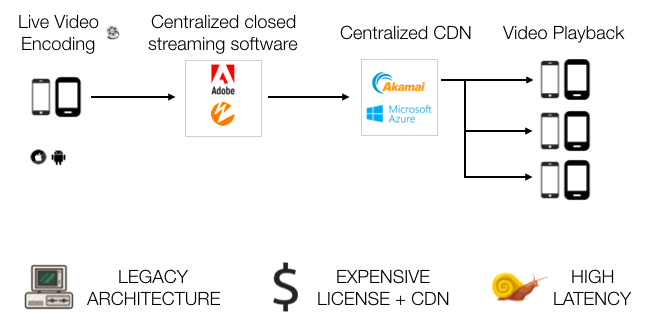
\includegraphics[width=1.0\textwidth]{static/problem-architecture-trans}
 \caption{Current closed, centralized, expensive, censorable live-streaming system}
 \label{image:problem-architecture-trans}
\end{figure}

Figure \ref{image:problem-architecture-trans} shows the state of current live-streaming system. There are 4 components to a live-streaming system. They are explained below.
\subsubsection{Broadcasting Software}
A proprietary mobile video encoding software is used. The primary purpose of this software is to capture video frames and audio, from mobile, desktop, or stand alone cameras. The software encode the captured video and audio frames into a video standard, and a closed/proprietary video streaming protocol and is published to Streaming software.

\subsubsection{Broadcasting Server Software}
Current software that solves this problem are Wowza\footnote{https://www.wowza.com/products} and Adobe\footnote{https://www.adobe.com/products/catalog.html}. The Broadcasting software receives the encoded live streams and generates small fragments of video files that are then published to a Content Delivery Network.

\subsubsection{Centralized Content Delivery Network}
The Broadcasting Server Software publishes the generated video fragment files to Content Delivery Network such as Amazon Cloud-front \footnote{https://aws.amazon.com/cloudfront/} or Microsoft Azure \footnote{https://azure.microsoft.com/en-us/services/media-services/}

\subsubsection{Video Player}
This is the final step in live video streaming. Media/Video/Audio clients for platforms: mobile, desktop, play out the video files from the content delivery networks.


These are the drawbacks with current live-streaming system:
\begin{itemize}
 \item[-]Centralized points of failures: Backend streaming software, relying on content delivery networks
 \item[-]Proprietary and closed source software
 \item[-]Prone to censorship as easy to control/shutdown the service
 \item[-]Expensive licensing fees
\end{itemize}

\subsection{GPUCoin Solution}
 % \fxerror{fix name for everything Hoot GPUCoin network, Hoot GPUcoin Token, Hoot GPUcoin protocol team, Hoot GPUcoin Foundation need right names for all and replace all }.

\begin{figure}[h!]
 \centering
 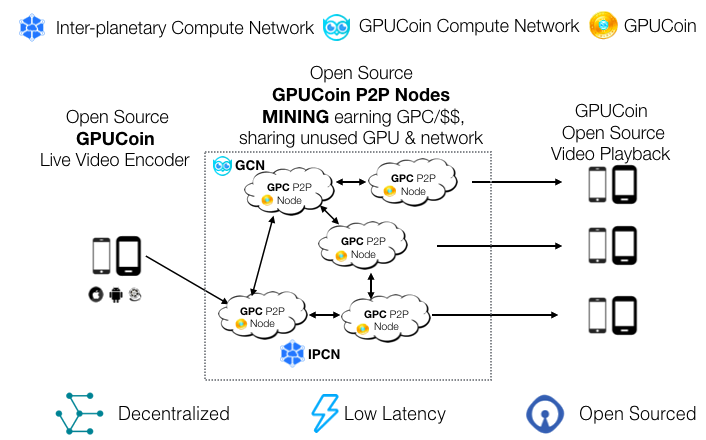
\includegraphics[width=1.0\textwidth]{static/gpucoin-solution-trans}
 \caption{Open Source, decentralized, censorship resistant Hoot live-streaming system}
 \label{image:gpucoin-solution-trans}
\end{figure}


Figure \ref{image:problem-architecture-trans} is the proposed live-streaming system. They are explained below.
\subsubsection{GPUCoin Open Source Broadcasting Software}
GPUCoin Open Source Broadcasting software captures video frames and audio. All major platforms: iOS, Android, Mac, Windows, Linux will be supported. The captured video frames and audio data are encoded to widely accepted open video and audio formats: H.264 and AAC. The encoded H.264 and AAC audio is published to the GPUCoin Network with Real Time Hoot Protocol(RTHP).

\subsubsection{GPUCoin P2P mining Node}
Miners in the GPUCoin GCN mining network P2P node will run GPUcoin software sharing unused bandwidth and earning GPUcoins for doing so. This is a highly resilient fault tolerant network, and miners will be able to join or leave the network anytime. The GPUCoin P2P Node replaces the need for a broadcasting server software and expensive content delivery network.

\subsubsection{GPUCoin Open Source Video player}
GPUCoin Open Source Video player plays the live stream in realtime. All major platforms: iOS, Android, Mac, Windows, Linux will be supported.

\subsubsection{Hoot archived videos}
Broadcasted video is continuously archived, and will be stored in decentralized file system IPFS. \footnote{Decentralized IPFS File system https://ipfs.io/} Hence GPUCoin live stream protocol makes the live-streaming faster, safer, and more open by
\begin{itemize}
 \item[+]having no single centralized points of failures - byzantine fault tolerant p2p network
 \item[+]Highly resilient fault tolerant network with peer to peer nodes
 \item[+]Censorship resistant as there are no centralized points of control
 \item[+]core peer to peer and networking software is open source
\end{itemize}

\section{What makes Hoot special}
When compared to other products on the market, Hoot has several defensible advantages:
\begin{itemize}
\item[*]Optimized for 2G/3G networks around the world, low CPU and GPU usage, saves battery and bandwidth consumption
\item[*]Next-gen live-streaming product that enables mobile phone self-serve streaming 
\item[*]Allows to interleave background music in a seamless manner
\item[*]Breakthrough patent-pending technology architected from the ground up requiring no licensing fees
\item[*]Hoot offers instant archival of live-stream videos making it unnecessary to upload files again at the end of livestream
\item[*]Modular architecture allows building Tor/VPN modules inorder to enable uncensorable live-streaming to promote free speech
\end{itemize}


\section{Traction \& Usage}
A mobile consumer application is currently live on the iOS AppStore and Google Playstore. Hoot has received streams from 

% \fxerror*{put right numbers}

Tables \ref{table:1} and \ref{table:2} show the usage statistics.

\setlength{\arrayrulewidth}{.7mm}
\setlength{\tabcolsep}{18pt}
\renewcommand{\arraystretch}{2.0} 
% \newcolumntype{s}{>{\columncolor[HTML]{AAACED}} p{3cm}}
% \arrayrulecolor[HTML]{DB5800}
 


\begin{table}[!htb]
\centering
\begin{tabular}{ |c|c| }
\hline
\rowcolor{lightgray} \multicolumn{2}{|c|}{User Statistics} \\
% \hline
% Metric Name & Metric Value \\
\hline
Monthly Active Users (MAU) & 214,769 \\
% \rowcolor{gray}
% Total Users & 3,000,000 \\
\hline
\end{tabular}
\caption{User Statistics}
\label{table:1}
\end{table}

\begin{table}[!htb]
\centering
\begin{tabular}{ |c|c| }
\hline
\rowcolor{lightgray} \multicolumn{2}{|c|}{Live Video Streaming Statistics} \\
% \hline
% Metric Name & Metric Value \\
\hline
Number of Videos & 48,207 \\
Average Viewers per stream & 155 \\
Average Stream Duration & 4 minutes 35 seconds \\
Total Time Watched & 37k days or 100 years \\
% \rowcolor{gray}
\hline
\end{tabular}
\caption{Live Video Streaming Statistics}
\label{table:2}
\end{table}


\iffalse
\section{Low Latency Streaming Technology}
\fxerror{maybe not needed}
How Hoot powers low latency streaming.
\fi

\section{Hoot Architecture}

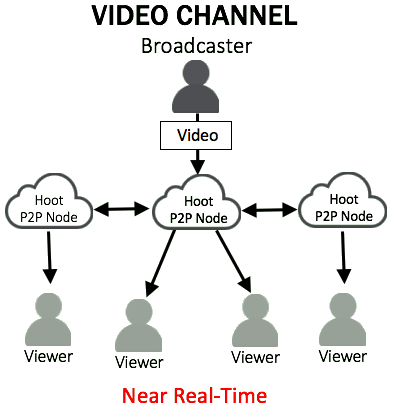
\includegraphics[scale=0.5]{static/hoot-video-architecture-channel-trans}

\subsection{Broadcast Side - mobile iOS client}
The protocol for realtime livestreaming video is called Real-Time Satoshi Streaming Protocol[\textbf{RTSSP}].
Video frames are captured at a resolution of 540x960 to 720x1280 based on network connectivity. Audio stream is captured using the built in iOS device microphone at a sampling rate of 44.1 KHz. Optionally, real time filters (Black and White, Glow, Fisheye, Sepia) can be applied to captured video frames in real-time. Video and audio are encoded using the native hardware H.264(H.265 in android) and AAC encoders, respectively. The video frames are encoded using a VBR algorithm with a maximum bitrate of 1 Mbps, this can be increased for usecases such as VR streaming. Audio stream is encoded in AAC format with a bitrate of 128 Kbps. The H.264 + AAC stream is encoded into an RTSSP stream and is transmitted to Hoot RTSSP server.

\subsection{Broadcast Side — Desktop Mac client}
Video frames are captured at native screen resolution, and audio stream is captured using the built in microphone at a sampling rate of 44.1 KHz. Hoot native cocoa Mac app written in Objective-C supports capturing FaceTime, Screenshare, and a combination of FaceTime and Screenshare. Video frames and audio stream are encoded using the native H.264 and AAC encoders, respectively. The video frames are encoded with a VBR algorithm. Audio stream is encoded in AAC format with a bitrate of 128 Kbps. The H.264 + AAC stream is encoded into an RTSSP stream and is transmitted to the open source RTSSP server.

\subsection{Viewer Side mobile iOS/Android client }
 Hoot open source Native mobile media player decodes RTSSP + H.264 and AAC data to make the live broadcast available to viewer in real-time. The HLS (HTTP Live Streaming) stream that is made available can be played using the iOS/Android Native media players, when the Hoot RTSSP player or app is not available.

\subsection{Viewer Side Mac/ Destkop PC client} 
The RTSSP stream is played using Adobe Flash technology supported by modern browsers. The HLS stream can be played using HTML5 player available in modern browsers.

\subsection{Server Side Peer-to-Peer decentralized Technology}
Similar to Bitcoin blockchain technology, any node can join or leave the Hoot network at anytime. Each node runs a realtime broadcasting server.
The GPUCoin network has several RTSSP servers that serve to bootstrap the Network. We use commodity servers with modern processors and with 1 Gbps duplex ethernet; specialized servers are not needed. The hoot server generates two variants of streams: a RTSSP stream and a HLS stream in order to make them accessible in browsers across Windows, Mac OS, Linux and Android platforms. A server with 1 Gbps duplex ethernet can support up to a total of 1000 viewers. A stream is replicated horizontally across multiple servers (without additional latency) to stream to virtually an unlimited number of simultaneous viewers. 

Streamed videos are instantly archived [\emph{H.264+AAC, mp4 container}] in the cloud for later viewing. The archived videos are indexed (scrubbable and quick to scan). We have access to datacenters in the following geographically distributed locations through RTSSP servers to provide the least latency to viewers globally: Amsterdam Netherlands, Frankfurt Germany, Hong Kong, London UK, Melbourne Australia, Queretaro Mexico, Milan Italy, Montreal Canada, Toronto Canada, Paris France, Singapore, Sydney Australia, Tokyo Japan, Dallas TX, Houston TX, San Jose CA, Seattle WA, Washington DC. 
% \sout{}
Streams are replicated and pulled to the closest node to the viewers location, i.e., a viewer in Tokyo Japan viewing a stream from Washington DC would be connected to a replicated stream on the Tokyo Japan hoot node in order to reduce latency.


%inlcude faster than input - input imports all commands http://i.imgur.com/YsPQMeD.png include{filename} gets you the speed bonus, but it also can't be nested, can't appear in the preamble, and forces page breaks around the included text by using \ clearpage before and after the content of the file.. 



\section{Security}
The live connection is encrypted using AES\_256\_CBC, with HMAC-SHA1 for message authentication and DHE\_RSA as the key exchange mechanism. Every Hoot opensource player connection is authenticated.
An authorization key is needed to view a private Hoot video stream. Signup, interactions, HLS streams and archived static content are end-to-end HTTPS SSL encrypted to ensure strong security. 

\subsection{Anonymity and privacy over VPN and Tor}
Anonymity and privacy are key to enable free speech, and this matters more in countries where free speech continues to be an ongoing human rights issue. In combination with blockchain technology, the network is
designed to route video streams and meta data over VPN and optionally Tor network to avoid censorship and promote free speech.

\section{GPUcoin Monetizing Engine}
GPUcoin tokens based on cryptocurrency technology power the Hoot marketplace and economy. Hoot miners earn GPUcoin tokens running their own open source decentralized Hoot nodes utilizing the unused networking bandwidth and compute capacity they may have. In countries where censorship is an issue they may run decentralized Hoot nodes with Tor/VPN modules enabled so they can support free speech through Hoot live-streaming. GPUcoin tokens can also be used by viewers to support their favorite artists, musicians and gamers. They may send GPUcoin tokens to the streamers they love watching and for events that they want to support. Streamers can also earn GPUcoin tokens by enabling subscriptions in order to have a dependable source of recurring revenue. This enables them to make a living off their fan base from the comfort of where they are at their best without having to spend for event space and the complicated offline co-ordinating schemes needed to assemble all their fan base for their events.

For micro-payments, artists can safely accept the HootLiveCoin payment immediately. The size of the payment is too small for the effort to steal it. Micro-payments are almost always for intellectual property, where there is no physical loss to the merchant.

 GPUcoin IPCN network will also build marketing and sales tool to help streamers and gamers market their events and build a paid subscriber base using email lists and sms lists among other social media channels. 
Musicians can also use the album selling tools to list and sell their albums, singles and release music videos. They can choose to exchange their GPUcoin tokens earned for crypto-currencies or fiat currencies.
 Streamers can also use GPUcoin tokens to purchase advertising space to feature events or utilize the marketing and sales tools to drive more viewers to their streaming events such as an album launch, book launch, movie launch or e-sports gaming event. Hoot miners, streamers and viewers can also load GPUcoin tokens on to their respective accounts using crypto-currencies such as Bitcoin, Ethereum, Litecoin, Monero, Zcash and fiat currencies such as USD, EUR among others.

\subsection{Hoot Augmented Reality ads - Performant AR ads with measurable ROI - Building Adwords of video }

Video Ads have been priced historically based on CPM for impressions as it has been nearly impossible to know how much of these video ads lead to a product sale/conversion or if they even positively affect the customer ROI. Viewers do not know what action to take and how to take the said action leaving them to figure out how to follow up on the video ad they just saw, leading to a lot of drop off and lack of performance of these video ads. Hence It’s not easy  to measure effectiveness and performance of the video ads historically.

Using interactive \textbf{Hoot AR} augmented reality  ads with clear
call to actions such as a buy button or rent button below the
interactive Hoot AR ad, sales can be generated right then and there,
after the viewer interacts with the Hoot AR ad. We will be able to
charge based on sales generated from the AR interaction i.e.,
referrals and instead of pricing based on CPM or impressions we can
price based on  cost per referral(\textbf{CPR}). The CPR price becomes
the signal that drives the continuous auction engine that powers the
Hoot ad marketplace. By bringing about an innovative CPR based
business model to video ads using Augmented reality
\emph{call-to-actions} we bring the effectiveness of Google AdWords to
video ads that only used to perform as well as banner ads
before. Hence Hoot AR ads, improves the effectiveness of plain video
ads, leading to a quantum improvement in video adspend ROI much like
AdWords improved the ROI of web based banner ads, laying the
foundation for a billion dollar ads business.


\section{Hoot video platform, plugins and video AppStore to support machine learning, augmented reality, VR and video v-apps}
We are quite excited by ARKit and ARCore which are going to be soon available in the upcoming versions of iOS11 and Android respectively. We believe this framework is going to usher a golden era of augmenting reality in video-streaming. With Tensor-flow, Caffe, Keras, Theano, TensorFlow Object Detection api, GCP cloud video intelligence API and Azure video machine-learning apis there is going to be a big wave of machine learning video content-analysis applications, makes videos searchable, and discoverable. You can now search every moment of every video file in your catalog and find every occurrence as well as its significance. Hoot video primitives via api/SDK will allow developers to extract actionable insights from video files without requiring any machine learning or computer vision knowledge. 

We envision an Augmented Reality first OS, an operating system native to virtual and augmented reality. We want to enable a thriving ecosystem by building a video appstore and provide a scalable platform for video developers around the world. By enabling a platform with easily extensible and scriptable plugins, and video appstore for AR and ML/AI v-apps, we will accelerate the golden age of intelligent live video and augmented reality. By providing an extensible plugin architecture, we will allow developers to build plugins on the Hoot video architecture. Filters, face-detection and face-swapping are some early augmented reality ideas that will be explored.
\iffalse
\sout{Some interesting machine-learning and ai ideas are Label Detection(Detect entities within the video, such as "dog", "flower" or "car"), Shot Change Detection (Detect scene changes within the video), Regionalization (automagically specify a region where processing will take place), automated subtitle detection, Home and office security and others yet to be discovered.} 
\fi

\subsection{Un-censorable P2P identity and reputation blockchain}
Since there is an economy of trading in the marketplace of the Hoot GPUCoin network, having a peer to peer identity and reputation database to enable seamless, non-custodial decentralized, trust-free interactions becomes essential. Users/Agents may be identified using Civic, UPort, or what the Decentralized Identity Foundation \footnote{http://identity.foundation} is building. Feedback and reviews as well as point scoring out of a maximum of 5 and minimum of 1 for quality of interactions factor into an agents reputation trust score. The trust score of each agent is hashed into the blockchain using their public GPG key and hashed username or decentralized identity so as to make them un-censorable. Trust score and reviews may only be added by anyone to the database and nothing can ever be removed making this the trust reputation blockchain. \emph{Merkle trees}, an efficient verifiable data-structure, is used to ensure the reputation db is usable by downloading the relevant sub-tree for a particular user sub-network hash even as the reputation blockchain grows very large in size as the network grows exponentially.

\subsection{Multi-sig escrow wallets}
GPUcoin tokens are first sent to a multi-sig escrow wallet, that is controlled by the buyer/viewer, seller/streamer and an independent third-party escrow. Any two out of the three parties need to sign in order for the transaction to be completed. Also the number of times the buyer or seller necessitates escrow agents to mediate a dispute and the time to complete a transaction will factor into the reputation of the buyer and seller. Any trusted agent with a high enough reputation score can register to be an independent third party escrow agent. Escrow agents also earn feedback and trust which are hashed and stored in the blockchain using their public GPG key and hashed username so it becomes un-censorable.


\subsection{Auction to find optimal price}
To bootstrap the network, GPUcoin IPCN network will run Vickrey auctions to find the best service to run on the miners computer that has excess capacity. A \emph{Vickrey auction} is one in which the winner pays the second-highest price, not the price they themselves bid, which has been effectively used by Google Adsense and Adwords.
Hoot can instantiate any auction protocol, if they find a suitable auction protocol that is superior to Vickrey. Its seed protocol specifies a procedure for stakeholders to approve amendments to the auction protocol,
\emph{including} amendments to the auction amendment procedure itself. Upgrades to Hoot auction protocol are staged through a testing environment to allow stake-holders and token-holders to recall potentially inferior amendments, that lead to sub-optimal pricing for network stakeholders. 

Since the Hoot GPUCoin network can also be used for other tasks than streaming live video, the network can be extended to run any computing task such as computer graphics, business applications, machine learning, cryptography, malware prevention analysis, science and services, making the GPUcoin IPCN network a Uber for computers, enabling miners to rent their unused CPU/GPU cycles and get paid in Hoot cryptocurrency. Hence the Hoot decentralized network powers true cloud computing.

\subsection{Cryptocurrency And Issuance}

The Hoot GPUcoin network includes its own built-in cryptocurrency, Hoot GPUcoins, which serves the dual purpose of providing a primary liquidity layer to allow for efficient exchange between various types of digital assets and, more importantly, of providing a mechanism for paying transaction fees.

The issuance model will be as follows:

\begin{itemize}

\item Hoot GPUcoins will be released in a cryptocurrency sale at the price of 1000-2000 Hoot GPUcoins per BTC, a mechanism intended to fund the Hoot organization and pay for development that has been used with success by other platforms such as Mastercoin, Filecoin, Ethereum, Tezos and NXT. Earlier buyers will benefit from larger discounts. The BTC, ETH, XMR, and LTC received from the sale will be used entirely to pay salaries and bounties to developers and invested into various for-profit and non-profit projects in the Hoot cryptocurrency ecosystem.

\end{itemize}

\subsection{Hoot-coin carbon footprint, mining, scarcity and profitability}
Bitcoin has made cryptocurrencies popular and brought it to the mainstream, but it has a dark side, its ever increasing carbon footprint. In late 2013, 8.25 megatons (8,250,000 tonnes) of CO$_2$ per year was estimated to be the carbon footprint of Bitcoin per year\footnote{https://pando.com/2013/12/16/bitcoin-has-a-dark-side-its-carbon-footprint/}. In August 2017, One Bitcoin transaction uses enough energy to power 5.58 US households for 1 day and the Bitcoin network consumes 30 times more energy than the VISA network \footnote{https://digiconomist.net/bitcoin-energy-consumption}. These computers are consuming so much electricity that it’s already unprofitable to mine in some regions of the world. Since excess bandwidth and compute capacity is utilized towards streaming, encoding, object recognition and security of video and audio streams the resources otherwise would be utilized are profitably used. Since GPUcoin tokens are fairly distributed to miners corresponding to their compute and bandwidth availability irrespective of how much CPU they control, the Hoot GPUCoin carbon footprint will be exponentially lower than the Bitcoin network which depends on continuously increasing complexity of the hashing required for mining. Since GPUcoin tokens can only be mined or acquired from the platform, they will tend to be a scarce token.

\section{The Foundation and Governance} % (fold)
\label{sec:the_foundation_and_governance}
As a company limited by guarantee established in Switzerland, the Hoot GPUcoin Foundation's primary objective is to promote the real world application of the Hoot Decentralized Open Live-Streaming platform. It also aims to initially develop the Hoot GPUcoin platform and advocate governance and transparency for the platform. The Hoot GPUcoin Foundation will establish an association consisting of members of the Hoot GPUcoin ecosystem, which will be empowered to determine the direction of functionality and improvement to the Hoot Live-Streaming platform and associated ecosystem.
% section the_foundation_and_governance (end)

\subsection{The dispute resolution process} % (fold)
\label{sub:the_dispute_resolution_process}
The Hoot GPUcoin Foundation will specify a dispute resolution process, utilizing an internationally accepted dispute resolution system. A rotating board of dispute referees will monitor disputes through the resolution process, and oversee collateral release to plaintiffs. Note that this board of dispute referees is not the dispute resolution process specifically; rather it is the mechanism through which dispute resolutions can be enacted through the release of collateral on the blockchain.


\subsection{Hoot GPUcoin Token sales} % (fold)
\label{sub:hoot_token_sales}
The Hoot GPUcoin Foundation will fund the development of the Hoot Live Stream Platform discussed in this paper through the issuance of Hoot GPUcoin tokens. These tokens will run natively on the Ethereum blockchain and will be offered to backers of the Hoot Live Stream project via a token sale. The token sale will be launched on or about the November 21 2017. A second token sale will take place once the initial prototype has been developed and tested to fund its deployment. 
\iffalse
For more information on the Hoot token, see \_\_\_ \fxerror{add correct section}.
\fi

\subsection{Token Allocation and Distribution} % (fold)
\label{sub:token_allocation_and_distribution}
 The supply of Hoot GPUcoin is limited to the number of one hundred million (100,000,000) in total (including those available for sale during the Token Sale) and will be generated upon the launch ("Token Launch".)

 The tokens will be distributed in the following manner:
60\% (30/30/20) of the tokens will be eventually allocated amongst the community; the remaining 20\% will be allocated to the Hoot GPUcoin Foundation initiator, early backers, and the Hoot GPUcoin protocol network development team.


\begin{table}[!htb]
\centering
\begin{tabular}{ |p{2.8cm}|p{2.5cm}|p{5cm}|}
\hline
\rowcolor{lightgray} \multicolumn{3}{|c|}{Hoot GPUcoin Token Distribution Model} \\
\hline
Channels & Percentage & Lock up Period \\
\hline
30,000,000 Hoot Hoot GPUcoin Token Sale (HTS) & 30\% & Token Sale - Launch 21 November 2017. The initial funding will be used to develop a working prototype, financial setup, legal fees and promotion.
 \\
 \hline
30,000,000 Hoot Additional Hoot GPUcoin Token Sale (AHTS) & 30\% & Additional Hoot GPUcoin Token Sale. On the release of a successful prototype, a second token sale will be launched to fund the full production ready launch and development of all relevant technology and organization matters.
\\
\hline
20,000,000 Hoot Retained by the Foundation as Treasury & 20\% & 100\% of which locked for 24 months.Strategic Planning, Project Support, Token Swap, Emergency Fund, Development \& Legal Fees - These will be subject to a 2 year lock-up. Subsequent to the lock-up, these will be used for various development and operation costs of Hoot Platform over 2 further years.
\\
\hline
20,000,000 Hoot GPUcoin Advisors, Directors and Early Backers & 20\% & 70\% of which is locked for 12 months. 30\% of which is locked up for 24 months. Distributed to the directors, advisors, and early backers of the
 project.
\\
 \hline
\end{tabular}
\caption{Hoot GPUcoin Token Distribution Model}
\label{table:hoot_token_distribution_model}
\end{table}
\iffalse
\fxerror{clean up table, better formatting/fonts}
\fi

\subsection{Restriction on the use of the funds} % (fold)
\label{sub:restriction_on_the_use_of_the_funds}
To remain in line with the spirit of the project’s open and transparent philosophy, all funds shall be tracked and reported according to the Foundation’s guidelines. A custodian will monitor the usage of the digital tokens and share it with the community periodically.

\begin{enumerate}
 \item Financial planning and reporting
 \begin{itemize}
 \item The Hoot GPUcoin Foundation shall develop financial planning and review financial performance of the previous quarter.
 \end{itemize}

 \item Digital tokens management
 \begin{itemize}
 \item The digital tokens belonging to the Foundation shall be managed by authorized personnel. The security of digital tokens is ensured by multi signature technology.
 \end{itemize}

 \item Digital wallet protocol
 \begin{itemize}
 \item The Foundation’s digital wallet shall be protected by a multiple signature technology mechanism.
 \end{itemize}

 \item Disclosure
 \begin{itemize}
 \item On a regular basis, the Foundation shall disclose on the topics regarding community matters, including status of development, operations, and the usage of tokens, as well as whether the Foundation operates in accordance with the governance policy.
 \end{itemize}
\end{enumerate}


\section{The Hoot GPUcoin Token}
The Hoot GPUcoin Token (HOOT) is a native Ethereum divisible digital token with up to 18 decimal places. The total number of GPUcoin tokens to be issued is 100,000,000. For details of the distribution of these tokens, see Section \ref{sub:token_allocation_and_distribution} \nameref{sub:token_allocation_and_distribution}.

\subsection{Uses of Hoot GPUcoin Token} % (fold)
\label{sub:uses_of_hoot_token}
Hoot GPUcoin token can be used for using the platform.
\iffalse
\fxerror{need to add economics of bandwidth sharing}
\fi
% subsection uses_of_hoot_token (end)
% subsection subsection_name (end)

\subsection{Insuring inflation rate does not outpace growth of underlying economy}
The sum total of all the Hoot GPUcoins coins minted at each interval can be guaranteed to be less than the calculated rate of economic growth similar to the variable bitcoin hashcash difficulty innovation, such that current token holders can be better assured that prices are not likely to inflate and that their tokens will fall below their original value because of an over inflation of excess Hoot GPUcoin token supply.

A further percentage of the growth can be retained as explained above to provide a price floor as an assurance of value maintenance to Hoot GPUcoin token holders. 

\section{Hoot GPUcoin Development Timeline}
The Hoot consumer mobile app which uses Facebook or Twitter to authenticate is already live in the iTunes AppStore\footnote{Hoot live on iOS AppStore https://appsto.re/us/40RS-.i} and Google Android Play Store\footnote{Hoot Live on Google Playstore https://play.google.com/store/apps/details?id=com.onhoot.android}.
A light weight performant native mac app is live on
the website \footnote{Download link for Hoot Live on Mac Desktop https://onhoot.com/mac}. The mac app can be used to screen-share meetings, conferences and webinars. It can also be used to livestream desktop games such as Minecraft, league of legends, world of warcraft and others.

A native enterprise version that uses Slack for authentication of internal private teams is already live.
 This requires quite a bit of work to integrate with the slack teams API and also in order ensure security for private teams. Following platforms are supported
\begin{itemize}

\item[-]iOS app for slack private teams \footnote{ iOS private Hoot business client for slack teams http://hootvideo.com/business}
\item[-]Hoot Mac desktop app for slack private teams \footnote{Desktop Hoot client for Slack teams http://hootvideo.com/macbusiness}
\item[-]All modern browsers. \footnote{Slack based private team build of Hoot https://hootvideo.com}
\end{itemize}

Web browser end points are live on line as well
\footnote{Hoot live link on Web browser https://onhoot.com}. The minimum requirements are any modern
browser such as Safari, Mozilla Firefox, Microsoft Internet Explorer or Google Chrome which fallback to HTML5 HLS video format for playback
of the live-streams.


\subsection{Tor and VPN to enable uncensorable live-streaming }
Tor modules to live-stream video over the onion routed tor network needs to be built. Integration with VPN needs to be built in order to evade censorship. This would enable true zero knowledge live-streams and computing in countries where censorships and free speech continue to be ongoing human rights issues.

The underlying Hoot technology may also be used to build an open source low cost security and surveillance alternative to closed systems such as Nest.

\subsection{Focus on Performance}
We have a strong focus on performance and highly performant applications while still maintaining smaller binary sizes and code integrity. The Hoot iOS app is under 10MB, the latency is under a second plus the network latency. This leads to a superior user experience and efficient usage of unused compute.

\section{Uber for Computers creating IPCN - Interplanetary compute network}
Hoot GPUcoin network is a dense Byzantine fault tolerant peer-to-peer network - creating the worlds first IPCN - Interplanetary compute network. Hoot GPUcoin Network is based on a complex architecture revolving around P2P, Blockchain, Smart Contracts, State Channels. Hoot GPUcoin network protocol will enable the creation of decentralized compute network, powered by decentralized cryptocurrency micro-payments. This leads to Uber for computers helping create the worlds first IPCN an interplanetary compute network. We will create a platform to create new compute primitives using any turing compute programming language. We will use container technologies such as docker and kubernetes to efficiently distribute and use excess unused compute. The compute results of the network are verifiable using cryptographic and mathematical properties of the cryptographic design. The IPCN takes advantage of the coming cambrian explosion of computing, cryptocurrencies and CPU/GPU miners.


\section{Conclusion}
Bet on the future with Hoot live-streaming protocol using GPUCoin for mining.


% \renewcommand{\lstlistingname}{Appendix}
% \begin{lstlisting}[caption={Digital Fingerprint},captionpos=b, language=java,numbers=none]

% {
% "$schema": "digital_fingerprint",
% "definitions": {},
% "id": "https://hootvideo.com/whitepaper",
% "properties": {
%  "compressedContent": {
%  "id": "/properties/compressedContent",
%  "items": {
%   "id": "/properties/compressedContent/items",
%   "type": "integer"
%  },
%  "type": "array"
%  },
%  "link": {
%  "id": "/properties/link",
%  "type": "string"
%  },
%  "name": {
%  "id": "/properties/name",
%  "type": "string"
%  },
%  "publishDate": {
%  "id": "/properties/publishDate",
%  "type": "string"
%  }
% },
% "type": "object"
% }

% \end{lstlisting}
\newpage
\listoffigures
\newpage 
\listoftables
\newpage 
\bibliographystyle{plain}
\end{document}

\end{lstlisting}

\bibliographystyle{plain}
\end{document}

